\section{La Belgian eID}

La carte d'identité électronique belge est entrée en vigueur en 2004. Elle comporte une carte à puce qui contient plusieurs informations quand au propriétaire de la carte. Elle permet au citoyen de s'authentifier mais également, pour les majeurs, de signer des documents. Elle comporte donc deux certificats: une d'authentification et un de signature (uniquement le premier pour les moins de dix-huit ans).

\subsection{But et fonctionnement}

Le but de l'intégration des eID au sein du projet est celui de permettre à l'utilisateur qui paie sur un site marchand de s'authentifier auprès de sa banque pour confirmer et valider le paiement. Pour faire cela il devra passer par les étapes suivantes: 

\begin{itemize}
    \item Entrer sa carte dans un lecteur de cartes
    \item Ouvrir l'application d'authentification eID
    \item Entrer son numéro de client après de la banque et le PIN de sa carte de crédit 
    \item  Signer avec son PIN de l'eID 
\end{itemize}

Par la suite de ces étapes, si toutes les informations sont correctes, le banque aura toutes les informations pour valider et donc autoriser le paiement. 

\subsection{Implémentation du module}

Le module d'authentification a été codé sous la forme d'une application Java, plus précisément utilisant
le JDK 19. Cette application client s'affiche au client grâce à une interface crée avec JavaFX. Le module
gère tout ce qui concerne la lecture de la carte elle-même mais également les échanges avec la
banque. Ces-derniers sont sécurisés via un chiffrement symétrique qui fonctionne via l'utilisation
d'une clé de session sur des Socket.
Le programme nécessite l'installation d'une DLL, nommée beidpkcs11.dll qui permet de s'interfacer et
de communiquer avec la carte. Cette DLL s'installe automatiquement lors de l'installation de
l'eIDViewer\footnote{https://eid.belgium.be/en}, un logiciel fourni par le Gouvernement Belge. Il est également nécessaire d'utiliser le
standard PKCS11, un protocole de cryptographie à clé publique. Dans notre cas, nous avons utilisé un
fichier de configuration standard fourni par les professeurs. Bien-sûr il faut également être en
possession d'un lecteur de carte, qui permettra de lire l'eID.
Une fois ce prérequis remplis, le client Java a tout ce dont il nécessite pour fonctionner.

\subsection{Fonctionnement pratique}

Il est évident que les échanges entre le Client et la Banque doivent être sécurisés, car les informations
qui transitent sur ces messages sont des données sensibles. Pour ces raisons, nous avons réfléchis à
un système qui permette d'assurer cette sécurité. Le diagramme qui suit illustre les premiers échanges
entre le Client, la Banque et le serveur de certificats.

\begin{figure}[H]
    \centering
    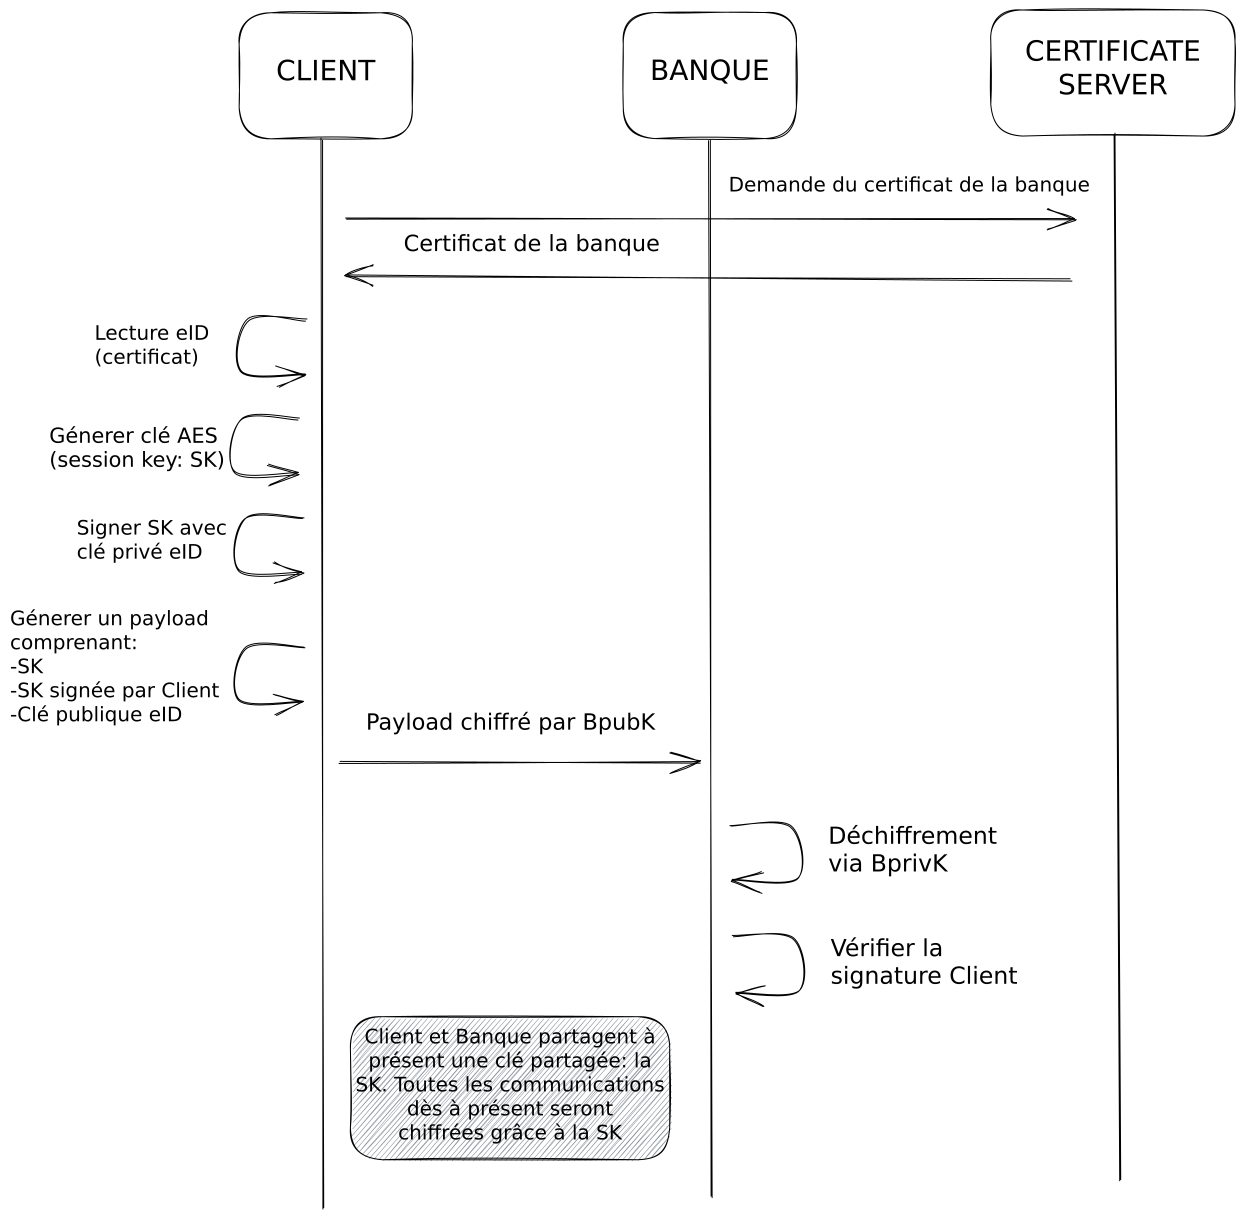
\includegraphics[width=\textwidth]{img/andrea-fig-1.png}
    \caption{Premiers échanges entre Client, Banque et Serveur de certificats}
    \label{fig:smartcard-exchange}
\end{figure}

Premièrement, le Client possède son certificat extrait de l'eID. Ceci lui donne accès à la clé publique
de son certificat, et à la clé publique. Cependant cette dernière n'est utilisable que pour la signature
de messages, et non pas pour chiffrer.
Nous constatons que les premiers échanges concernent le partage des clé publiques, et le plus
important, la création d'une clé de session. Celle-ci nous permettra de chiffrer les futurs échanges
entre Client et Banque. La clé de session (\textbf{SK}) est générée du côté du Client, qui s'occupe également de la signer, pour prouver son authenticité à la banque. De plus il envoie également sa clé publique à
la Banque, pour que celle-ci puisse vérifier cette signature. Ces trois blocs d'information sont envoyés
en un seul message chiffré avec la clé publique de la Banque. Ceci signifie que seule la Banque pourra
le déchiffrer.

Dès à présent, tous les futurs messages seront chiffrés via la clé de session, qui a été échangée entre
Client et Banque de manière sécurisée. Maintenant débute la véritable vérification qui autorisera le
paiement.

\begin{figure}[H]
    \centering
    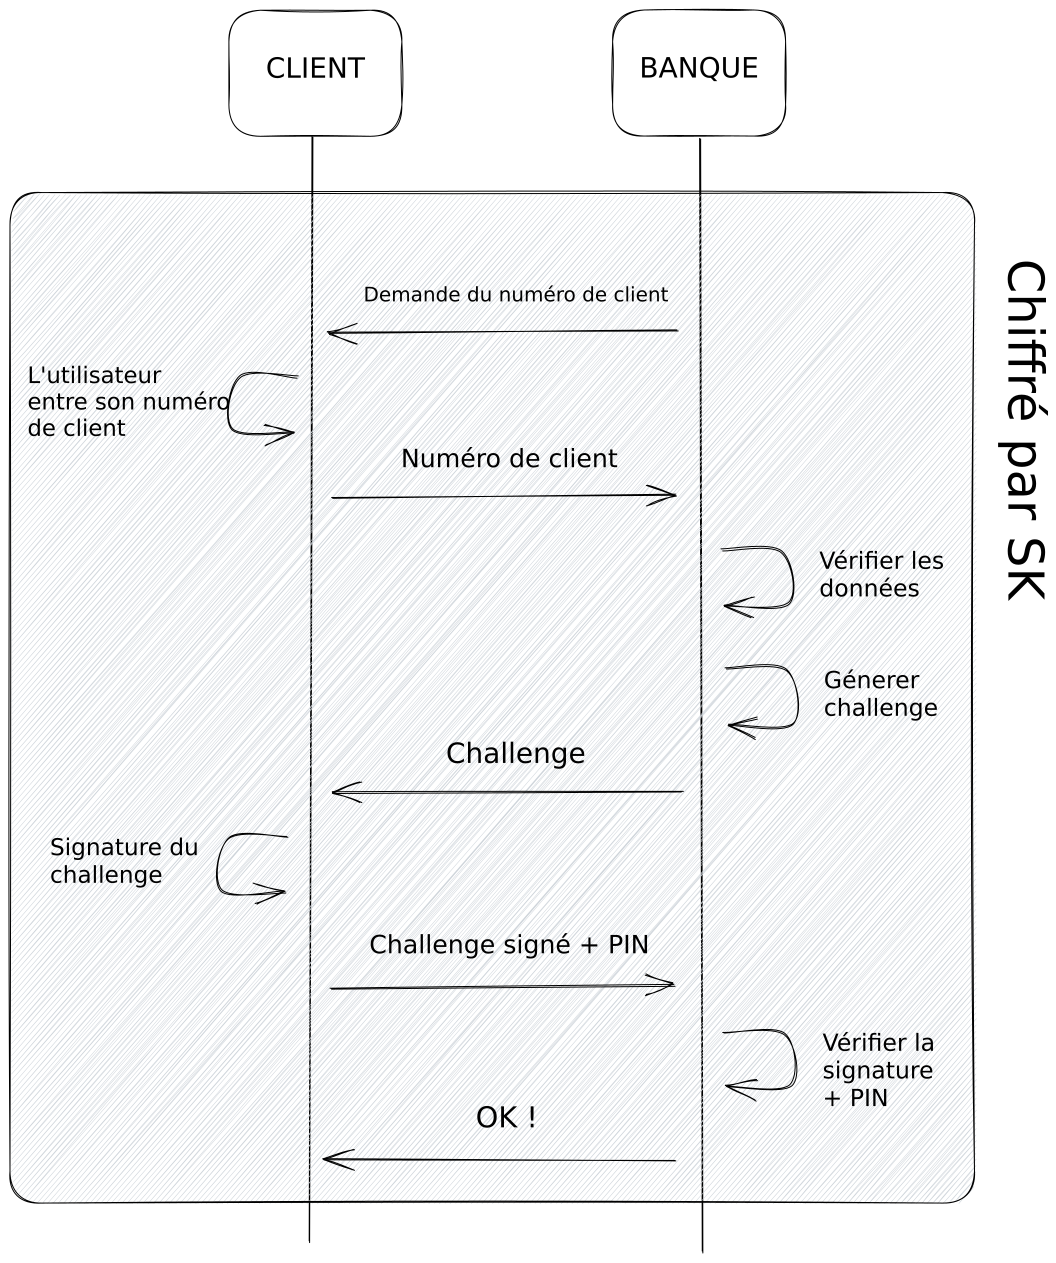
\includegraphics[scale=.5]{img/andrea-fig-2.png}
    \caption{Seconde phase de l'authentification}
    \label{fig:smartcard-exchange02}
\end{figure}

En cette seconde phase, nous traitons les données plus sensibles, d'où la nécessité du chiffrement
garanti par notre clé de session. Une fois que la banque reçoit le numéro de client demandant
autorisation, elle générera un challenge, qui sera signé par le client. Lorsque cette signature est
vérifiée, le paiement est autorisé et l'échange se termine.

\section{Gestion de points de fidélité par smartcard}

Pour cette tâche, nous avons utilisé la technologie Java Card, présentée au cours de Smartphone et
Cartes à Puces. Pour des raisons de simplicité, de respect de l'environnement et de limitations
d'infrastructure, nous nous sommes limités à l'utilisation d'un simulateur de Java Card plutôt
qu'investir dans du réel matériel dont l'utilisation future pourrait n'être que fortement limitée.
Les points de fidélité trouvent confortablement leur place au sein du projet intégré dans le cadre d'une
gamification de l'expérience d'achat, qui, dans un cas plus développé du projet, pourrait donner la
possibilité à l'acheteur de bénéficier de réductions et avantages.

\subsection{But et fonctionnement}

Le cartes de fidélité fonctionnent de paire avec les sites et bases de données marchandes. Ces
dernières gardent une traces des achats d'un client. Sur base de ses achats, il accumulera un certain
nombre de points. Ces points sont calculés automatiquement du côté des marchands. Le cartes de
fidélité entrent en jeu lors des achats faits physiquement en magasin. Par exemple, lors d'une
promotion spéciale, le client a droit à 50\% plus de points pour ses achats en magasin. Ceci est géré
donc par la petite application crée pour ce projet. L'utilisateur, qui sera de fait le responsable de caisse
ou autre travailleur du marchand, scannera la carte de fidélité et aura la possibilité d'ajouter un certain
nombre de points pour le client. Un autre cas pourrait être l'échange des points pour une réductions
sur le total des achats. Dans ce cas, le responsable pourra aussi soustraire des points de la carte. Toutes
ces manipulations sont reflétées dans la base de données qui sera notifié et mise à jour à chaque
changement sur la carte.

\subsection{Fonctionnement du module}

Concrètement, l'application est matérialisée par une application Java, qui fonctionne en mode console.
L'absence d'une interface graphique a été due à des difficultés rencontrés à cause d'une incompatibilité
entre la version de Java nécessaires au bon fonctionnement de certaines librairies qui s'interfacent
avec les cartes Java Card. Le module est séparé en deux parties.
La première, qui constitue le cœur de la Java Card est l'applet. Cette partie a été codée sur la version
7 de Java et en utilisant le JCDK (Java Card Development Kit). L'applet défini la véritable structure de la
carte et défini non seulement les données qu'elle contiendra mais également les opérations que celle-
ci peut opérer. Dans notre cas, nous stockons simplement deux informations sur la carte : un identifiant
du propriétaire et le total de ses points. A côté de cela, les opérations qui sont stockées sur la carte
concernent la lecture et l'écriture de ces variables. D'autres méthodes supplémentaires permettent de remettre à zéro les total des points, de réattribuer le propriétaire de la carte et de reset la carte
totalement. Cette applet est donc compilée grâce au JCDK (Java Card Development Kit) et écrit dans la
mémoire EEPROM de la carte à puce.

\begin{listing}[H]
    \begin{minted}{java}
        public class AppletProjetIntegre extends Applet {
            /******************* Constantes ****************/
            public static final byte CLA_PROJECTAPPLET = (byte) 0xB0;
            public static final byte INS_GET_POINTS = 0x00;
            public static final byte INS_SET_POINTS = 0x01;
            public static final byte INS_RES_POINTS = 0x02;
            public static final byte INS_GET_ID = 0x03;
            public static final byte INS_SET_ID = 0x04;
            public static final byte INS_RES_ID = 0x05;
            public static final byte INS_RES_CARD = 0x06;
        
            /**************** Variables *******************/
            private byte id;
            private byte points;

            private AppletProjetIntegre() {
                id = 0;
                points = 0;
            }

            /*
                ...
            */
        }
    \end{minted}
    \caption{Définition des variables et des fonctions présentes sur la Java Card}
    \label{listing:applet-projet-integre}
\end{listing}

La seconde partie du client est le programme qui s'interface à la carte et l'interroge. Les méthodes
définies dans l'applet via des codes hexadécimaux sont réutilisées dans ce même projet, qui utilise les
codes pour échanger des informations avec la carte. Ici est également cachée la logique qui appelle
l'API du marchand.
Dès l'insertion de la carte, le programme vérifie d'abord qu'un identifiant est bien présent sur la carte.
Le cas échéant, le programme demande d'attribuer la carte à quelqu'un. Le responsable dans ce cas
entre le nom ou l'email du client, et, si celui-ci est enregistré dans la base de données du marchand, la
carte est initialisée avec les l'identifiant du nouveau propriétaire et ses points actuels sont également
écrits. Une fois la carte prête, le responsable a la possibilité d'ajouter, de soustraire ou de simplement
consulter le nombre de points disponibles sur la carte.

\section{Conclusions personelles}

Du point de vue personnel, ce projet fut un grand défi, tant du point de vue technique, que de celui
d'organisation. Le déroulement du projet s'est bien passé grâce à une bonne ambiance et une bonne
entente au sein du groupe.
Du point de vue technique, la partie eID a sans doute été le plus grand défi. L'absence de réelle
documentation ont rendu le développement d'autant plus lent et souvent basé sur du « trial and
error ». Cependant cela a résulté en une bonne compréhension du fonctionnement des carte
d'identité électroniques et sur les possibilités qu'elles offrent. La partie Java Card, s'est déroulé avec
moins de difficultés, du moins pour la programmation de l'applet.
Du point de vue de l'organisation, la plus grande difficulté rencontré a été celle de l'organisation du
travail au sein de l'équipe et la répartition des tâches. Nous avions initialement pensé que la partie eID
et Java Card était plutôt isolé du reste du projet et cela est vrai, mais uniquement partiellement. J'ai
personnellement dû me coordonner avec d'autre membres du groupe pour compléter des parties de
mon travail, et j'ai essayé d'aider quand cela m'était possible.
Globalement, j'estime que nous avons tous beaucoup appris sur les projets en équipe, sur les difficultés
qu'ils présentent et sur la manière de les affronter. Si nous devions recommencer le projet, nous
porterions sans doute une attention plus importante quant à la définition plus précise de sprint et à la
répartition des tâches, qui dans le cas de notre groupe a parfois été sous-optimale
